\section{Chebyshev and Lagrange interpolation}

In the following functions, the domains are defined for all $\delta>0$ or $r>0$, so in finding Chebyshev nodes for interpolation, only nodes
in this domain are filtered from a list of possibilities. Thus, when selecting $n$ nodes, we actually select more, of which the negative values are discarded.
Using the Lagrange polynomial interpolation method, these nodes are used to find an approximating polynomial.

\subsection{Interpolation of \texorpdfstring{$\phi_0,\phi_\mathrm{min}$}{}}

In Figure \ref{phi0lg} and \ref{phimlg}, 9 Chebyshev nodes were used to generate an approximating polynomial.

\begin{figure}[H]
    \centering
    \begin{minipage}{0.45\textwidth}
        \centering
        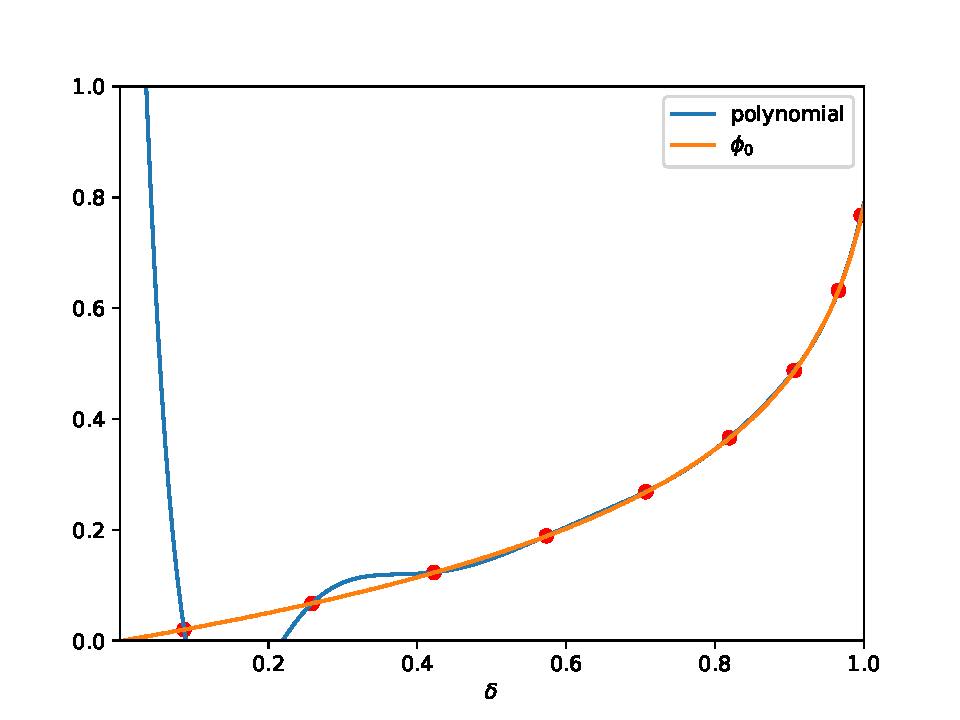
\includegraphics[scale=0.45]{plots/phi0_lagrange.pdf}
        \caption{Lagrange polynomial approximation of $\phi_0$ with equation $g$}\label{phi0lg}
    \end{minipage}\hfill
    \begin{minipage}{0.45\textwidth}
        \centering
        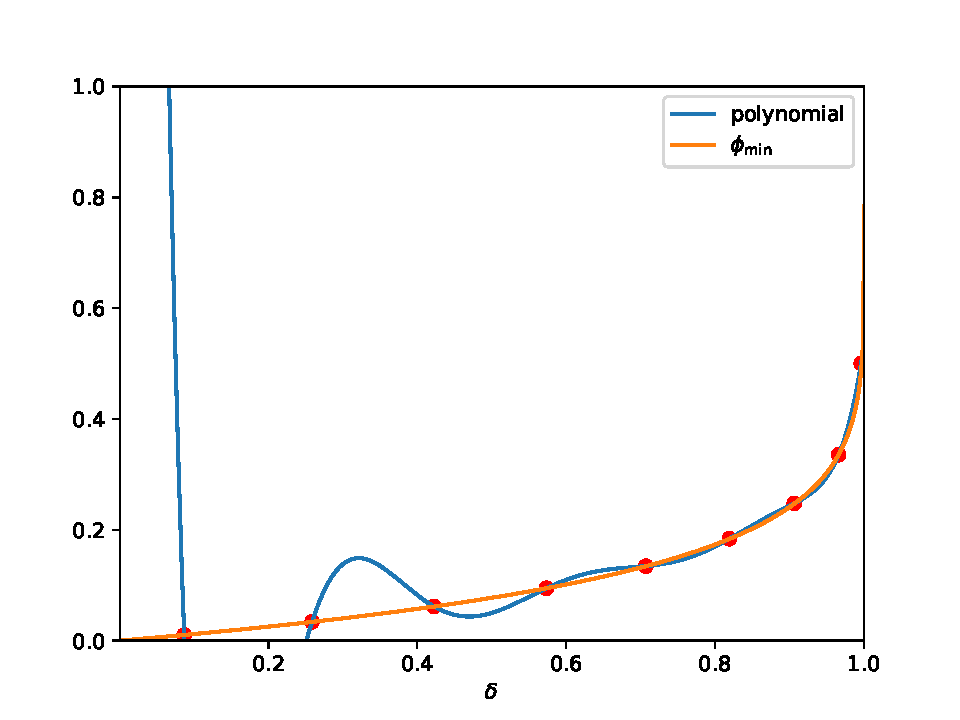
\includegraphics[scale=0.45]{plots/phimin_lagrange.pdf}
        \caption{Lagrange polynomial approximation of $\phi_\mathrm{min}$}\label{phimlg}
    \end{minipage}
\end{figure}

Polynomial for $\phi_0$:

\begin{equation}
    f_1(\delta)=1044\delta^{8}-4892\delta^{7}+9693\delta^{6}-10531\delta^{5}+6800\delta^{4}-2638\delta^{3}+589\delta^{2}-67\delta^{1}+3
\end{equation}

Polynomial for $\phi_\mathrm{min}$:

\begin{equation}
    f_2(\delta)=3968\delta^{8}-18749\delta^{7}+37405\delta^{6}-40874\delta^{5}+26519\delta^{4}-10327\delta^{3}+2311\delta^{2}-263\delta^{1}+11
\end{equation}

The coefficients displayed here are rounded to the nearest whole number in order to make for readable output.

\subsection{Interpolation of \texorpdfstring{$y(r)$}{}}

As shown in Figure \ref{yrpoly}, the Cheybshev node method yielded far more accurate results for the function $y(r)$, save for the initial spike/irregularity in the function when it is increasing.

\begin{figure}[H]
    \centering
    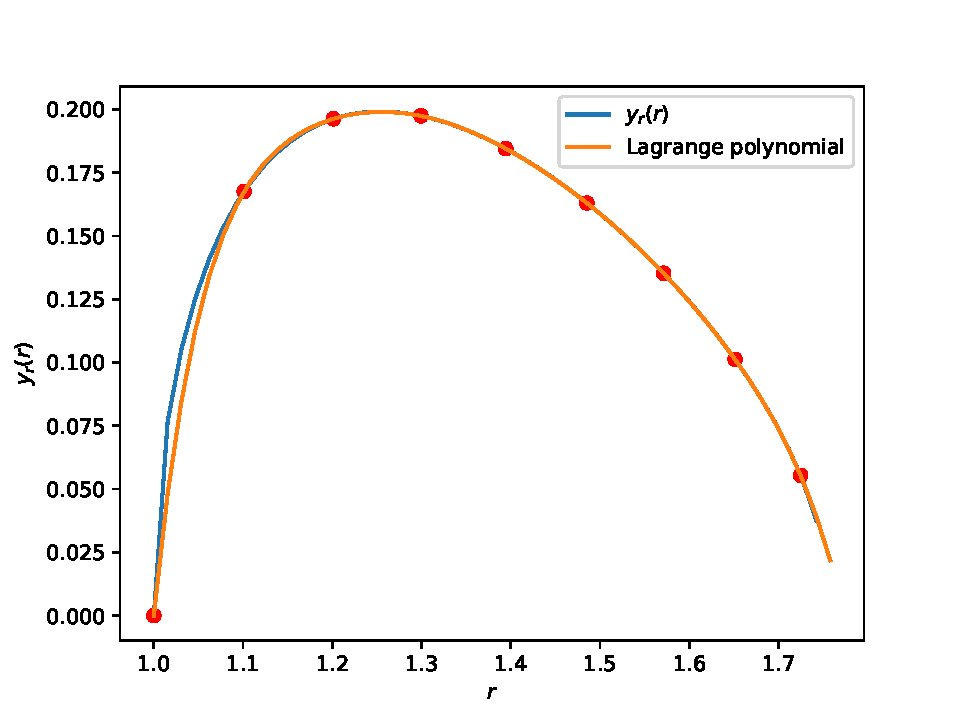
\includegraphics[scale=0.8]{plots/yr_poly.pdf}
    \caption{Lagrange polynomial approximation for $y(r)$}\label{yrpoly}
\end{figure}

The equation of the Lagrange polynomial is:
\begin{equation}
    f_3(r)=-282r^{8}+3195r^{7}-15828r^{6}+44706r^{5}-78750r^{4}+88591r^{3}-62158r^{2}+24872r^{1}-4346
\end{equation}

\subsubsection{Integral approximation for \texorpdfstring{$\frac{dr}{dt}=y(r)$}{}}

The definition given is $y(r)=\frac{dr}{dt}$. This can be rearranged to

\begin{equation}
    \frac{dr}{y(r)}=dt
\end{equation}

Taking the indefinite integral on both sides (the limit on the side with $r$ is from $r_0=1$ to $r_m$ where $y(r_m)=1|r_m > 1$ and from $0$ to some $t_f$ for the side with $t$) we get

\begin{equation}
    \int_{1}^{r_m}\frac{dr}{y(r)}=\int_0^{t_f}dt
\end{equation}

Using the approximation in Eq. 30, this becomes

\begin{equation}
    \int_{1}^{r_m}\frac{dr}{f_3(r)}=\int_0^{t_f}dt
\end{equation}

Using an optimized solver, the unknown is $t_f=4.52624262$.

\subsection{Limitations and future goals}

\begin{itemize}
    \item The NumPy Lagrange solver does not allow for specification of some tolerance $\epsilon$
    \begin{itemize}
        \item A potential solution could be to implement the Lagrange polynomial method from scratch, where a tolerance could be specified
    \end{itemize}
    \item Another interpolation routine that could be used is the Newton polynomial method, which could also be implemented manually in order to specify a tolerance
\end{itemize}